\documentclass{article}
%cmd + shift + P
\usepackage{fontspec}   %加這個就可以設定字體
\usepackage{csvsimple}

\usepackage{xeCJK}       %讓中英文字體分開設置
\usepackage[T1]{fontenc}
\usepackage{bigfoot} % to allow verbatim in footnote
\usepackage[numbered,framed]{matlab-prettifier}
\usepackage{graphicx}
\usepackage{filecontents}
\graphicspath{ {img_hw1/} }
% \setCJKmainfont{標楷體} %設定中文為系統上的字型,而英文不去更動,使用原TeX字型
% \XeTeXlinebreaklocale "zh"             %這兩行一定要加,中文才能自動換行
% \XeTeXlinebreakskip = 0pt plus 1pt     %這兩行一定要加,中文才能自動換行
\title{\emph{生醫工程實驗, Spring 2017}\\ Lab3 超音波醫學影像分析(Ultrasound)}
\author{第五組\ 蔡承佑\ 許博竣\ 許秉鈞}
\date{May 24, 2017} %日期
\let\ph\mlplaceholder % shorter macro
\lstMakeShortInline"

\lstset{
  style              = Matlab-editor,
  basicstyle         = \mlttfamily,
  escapechar         = ",
  mlshowsectionrules = true,
}

\begin{document}
\maketitle


\section{Point Spread Function(PSF)}
\subsection{實驗原理}

點擴散函數(point spread function, 簡稱 PSF)。是描述光學系統對點源解析能力的函數。因點源在經過任何光學系統後都會由於衍射而形成一個擴大的像 點。通過測量系統的點擴展函數,能更準確地提取圖像信息。而 PSF 與 impulse response 有相同的概念。

\subsection{實驗數據}
\emph{a) Estimate PSF size for In-focused and Out-focused targets}  \\
以下用 5.7cm, 7.1cm 深度、 pen/res 模式來測量\\
\\
\emph{b) Repeat (a) under different B-mode gain} \\

\pagebreak
\begin{itemize}
\item{\emph{5.7cm/high gain/pen}}
\begin{center}
\csvautotabular{img_hw1/57-high-pen.csv}
\end{center}
\begin{figure}[h]
    \centering
    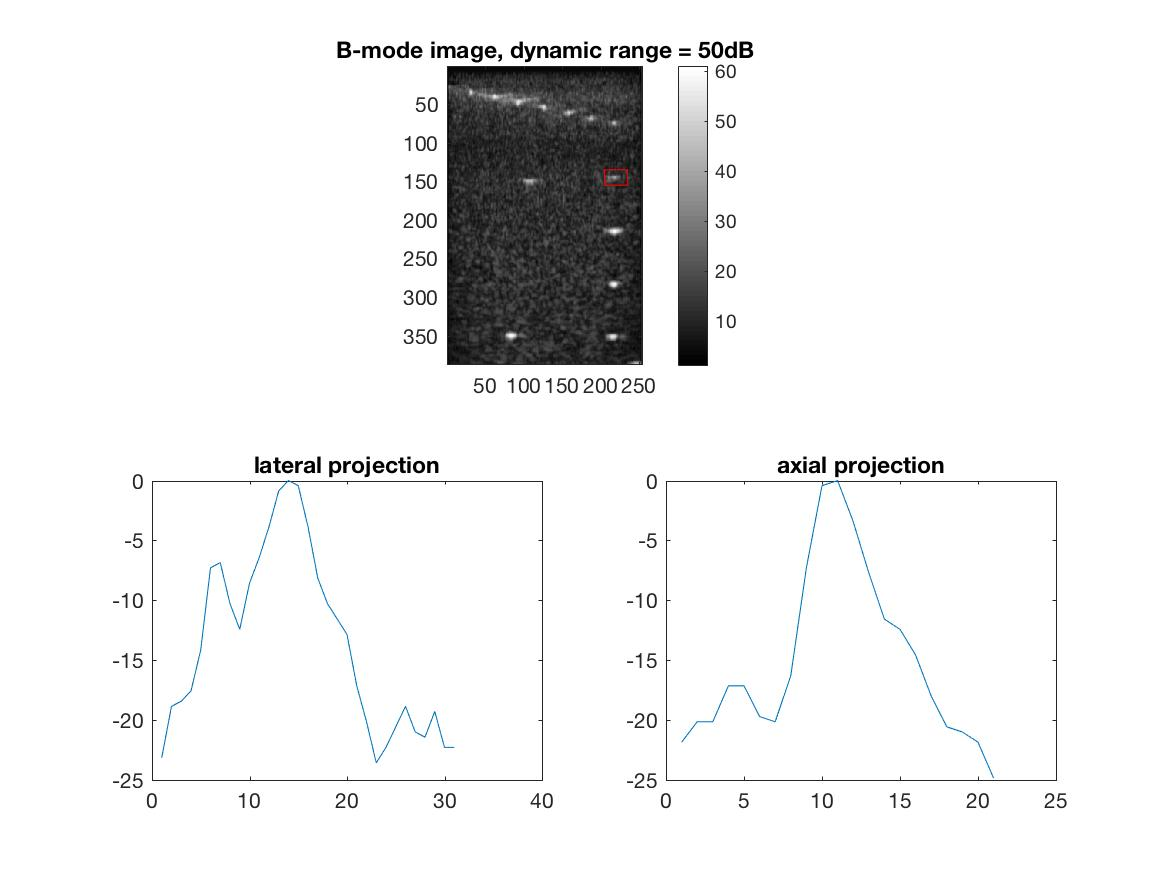
\includegraphics[width=1.0\textwidth]{img_hw1/57-high-pen1.jpg}
    \caption{57-high-pen(In Focus)}
    \label{fig:mesh1}
\end{figure}
\pagebreak
\begin{figure}[h]
    \centering
    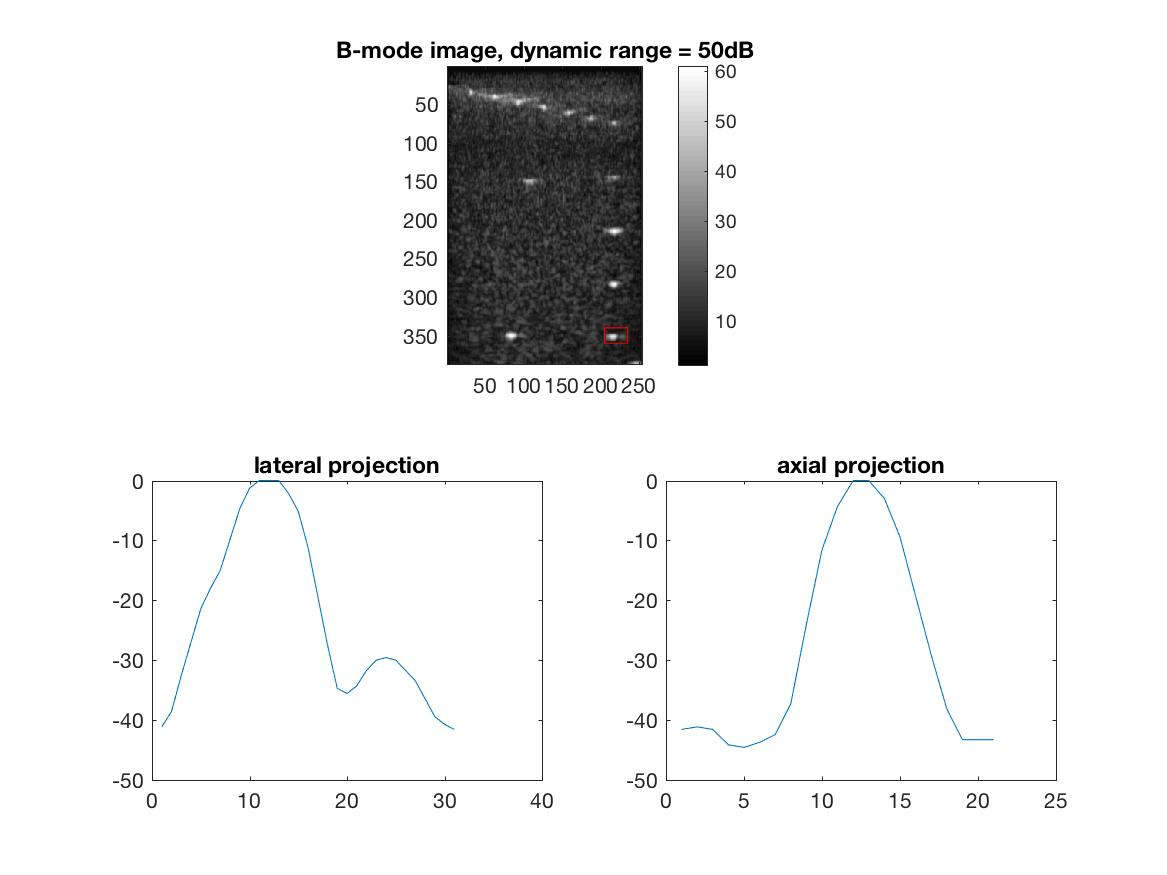
\includegraphics[width=1.0\textwidth]{img_hw1/57-high-pen2.jpg}
    \caption{57-high-pen(Out Focus)}
    \label{fig:mesh1}
\end{figure}
\item{\emph{5.7cm/high gain/res}}
\begin{center}
\csvautotabular{img_hw1/57-high-res.csv}
\end{center}
\end{itemize}



\end{document}
